\chapter{Image classification}


\section{Supervised datasets}

\begin{description}
    \item[Dataset] \marginnote{Dataset}
        Given a set of labeled data, it can be split into:
        \begin{descriptionlist}
            \item[Train set] $D^\text{train} = \{ (\text{x}_\text{train}^{(i)}, y_\text{train}^{(i)}) \mid i = 1, \dots, N \}$.
            \item[Test set] $D^\text{test} = \{ (\text{x}_\text{test}^{(i)}, y_\text{test}^{(i)}) \mid i = 1, \dots, M \}$.
        \end{descriptionlist}

        It is assumed that the two sets contain i.i.d. samples drawn from the same unknown distribution.
\end{description}


\subsection{Modified NIST (MNIST)}

\begin{minipage}{0.45\linewidth}
    \centering
    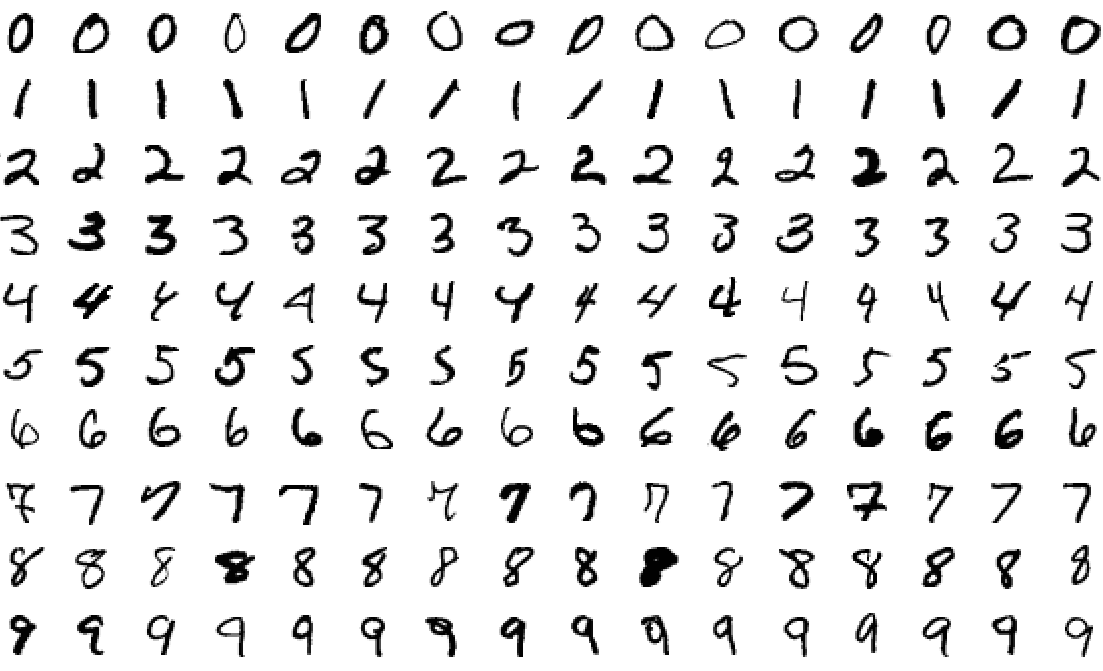
\includegraphics[width=0.9\linewidth]{./img/mnist.png}
\end{minipage}
\begin{minipage}{0.5\linewidth}
    \begin{descriptionlist}
        \item[Content] Handwritten digits from 0 to 9.
        \item[Number of classes] 10.
        \item[Train set size] 50k.
        \item[Test set size] 10k.
        \item[Image format] $28 \times 28$ grayscale.
    \end{descriptionlist}
\end{minipage}


\subsection{CIFAR10}

\begin{minipage}{0.45\linewidth}
    \centering
    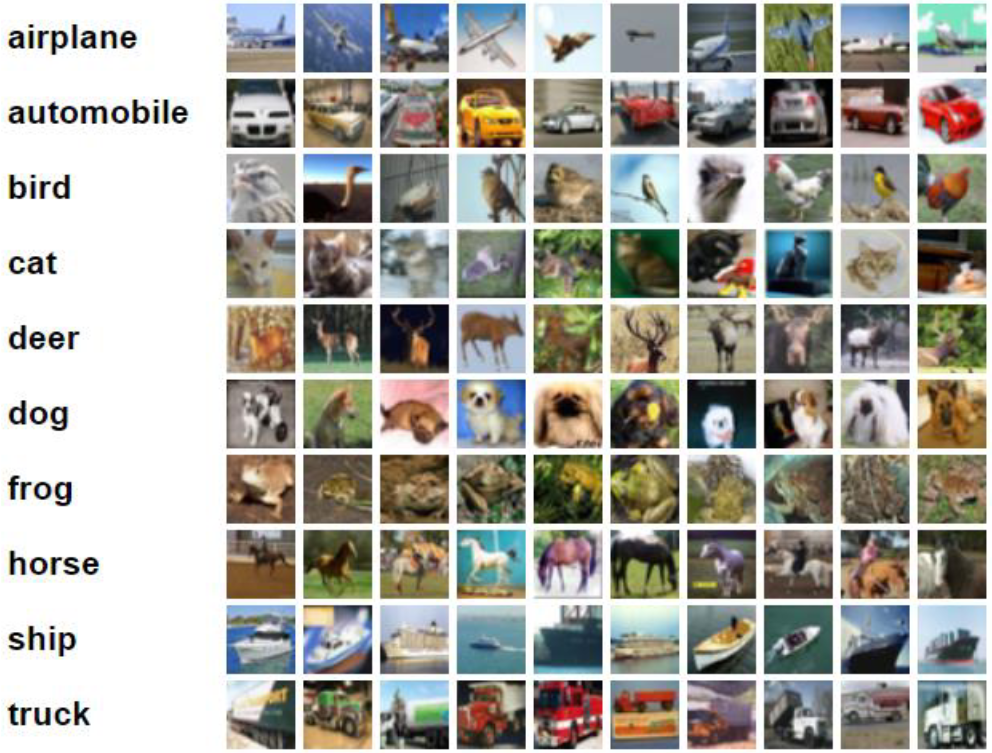
\includegraphics[width=0.9\linewidth]{./img/cifar10.png}
\end{minipage}
\begin{minipage}{0.5\linewidth}
    \begin{descriptionlist}
        \item[Content] Objects of various categories.
        \item[Number of classes] 10.
        \item[Train set size] 50k.
        \item[Test set size] 10k.
        \item[Image size] $32 \times 32$ RGB.
    \end{descriptionlist}
\end{minipage}


\subsection{CIFAR100}

\begin{minipage}{0.45\linewidth}
    \centering
    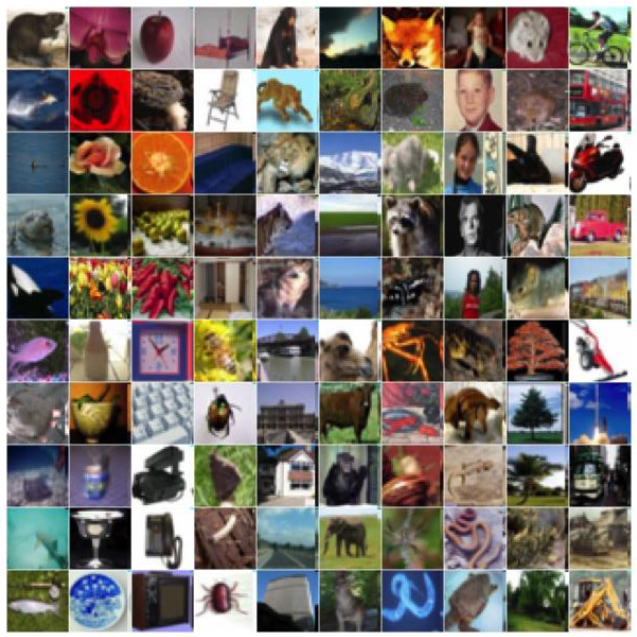
\includegraphics[width=0.7\linewidth]{./img/cifar100.png}
\end{minipage}
\begin{minipage}{0.5\linewidth}
    \begin{descriptionlist}
        \item[Content] Objects of various categories.
        \item[Number of classes] 100 (20 super-classed with 5 sub-classes).
        \item[Train set size] 50k.
        \item[Test set size] 10k.
        \item[Image size] $32 \times 32$ RGB.
    \end{descriptionlist}
\end{minipage}


\subsection{ImageNet 21k}

\begin{descriptionlist}
    \item[Content] Objects of various categories.
    \item[Number of classes] 21k synsets from WordNet organized hierarchically.
    \item[Dataset size] 14 millions.
    \item[Image size] Variable resolution RGB. Average size of $400 \times 350$.
\end{descriptionlist}

\begin{figure}[H]
    \centering
    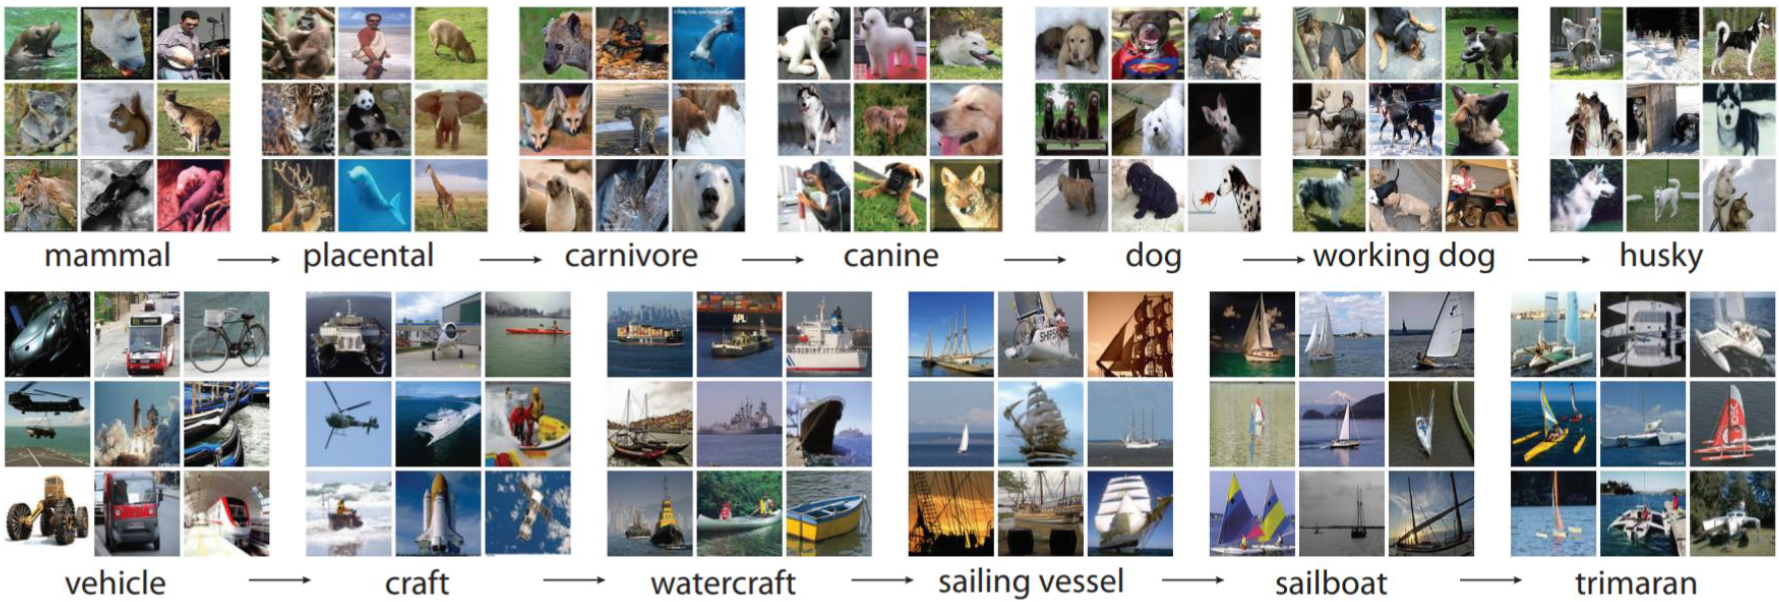
\includegraphics[width=0.85\linewidth]{./img/imagenet21k.png}
\end{figure}


\subsection{ImageNet 1k}

\begin{minipage}{0.45\linewidth}
    \centering
    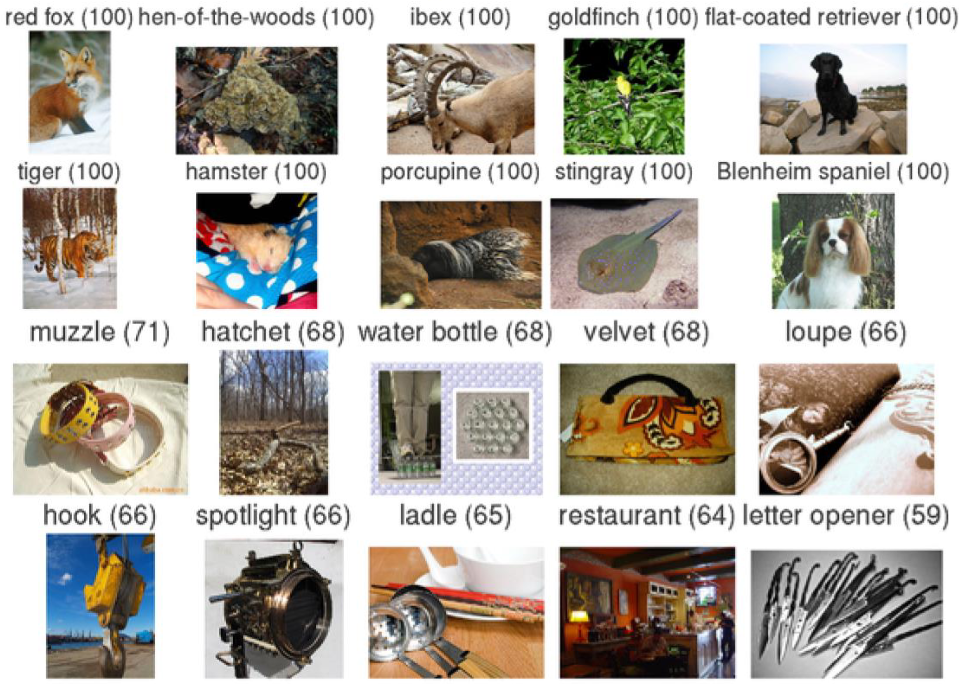
\includegraphics[width=\linewidth]{./img/imagenet1k.png}
\end{minipage}
\begin{minipage}{0.5\linewidth}
    \begin{descriptionlist}
        \item[Content] Objects of various categories.
        \item[Number of classes] 1000.
        \item[Train set size] $1.3$ millions.
        \item[Validation set size] 50k.
        \item[Test set size] 100k.
        \item[Image size] Variable resolution RGB. Often resized to $256 \times 256$.
    \end{descriptionlist}
\end{minipage}

\begin{remark}
    Performance is usually measured as top-5 accuracy as making a single prediction might be ambiguous due to the fact that the images can contain multiple objects.
\end{remark}



\section{Learning}

\begin{description}
    \item[Learning problem] \marginnote{Learning problem}
        Find the best model $h^*$ from the hypothesis space $\mathbb{H}$ that minimizes a loss function $\mathcal{L}$:
        \[ h^* = \arg\min_{h \in \mathbb{H}} \mathcal{L}(h, \matr{D}^\text{train}) \]

        In machine learning, models are usually parametrized. The problem then becomes to find the best set of parameters $\matr{\theta}^*$ from the parameter space $\Theta$:
        \[ \matr{\matr{\theta}}^* = \arg\min_{\matr{\theta} \in \Theta} \mathcal{L}(\matr{\theta}, \matr{D}^\text{train}) \]
\end{description}


\subsection{Loss function}

\begin{description}
    \item[Loss function] \marginnote{Loss function}
        Easy to optimize function that acts as a proxy to measure the goodness of a model.

        The loss computed on a dataset is usually obtained as the average of the values of the single samples:
        \[ \mathcal{L}(\matr{\theta}, \matr{D}^\text{train}) = \frac{1}{N} \sum_{i}^{\vert \matr{D}^\text{train} \vert} \mathcal{L}\big( \matr{\theta}, (\vec{x}^{(i)}, y^{(i)}) \big) \]


    \item[0-1 loss] \marginnote{0-1 loss}
        Loss computed as the number of misclassifications:
        \[ \mathcal{L}\big( \matr{\theta}, (\vec{x}^{(i)}, y^{(i)}) \big) = \vert \text{misclassifications} \vert \]

        This loss is not ideal as it is insensitive to small (or even large) changes in the parameters.
        Moreover, it does not tell in which direction should the parameters be modified to reduce the loss.

        \begin{remark}
            This loss can be minimized using a combinatorial optimization approach but it does not scale well with large datasets.
        \end{remark}

        \begin{figure}[H]
            \centering
            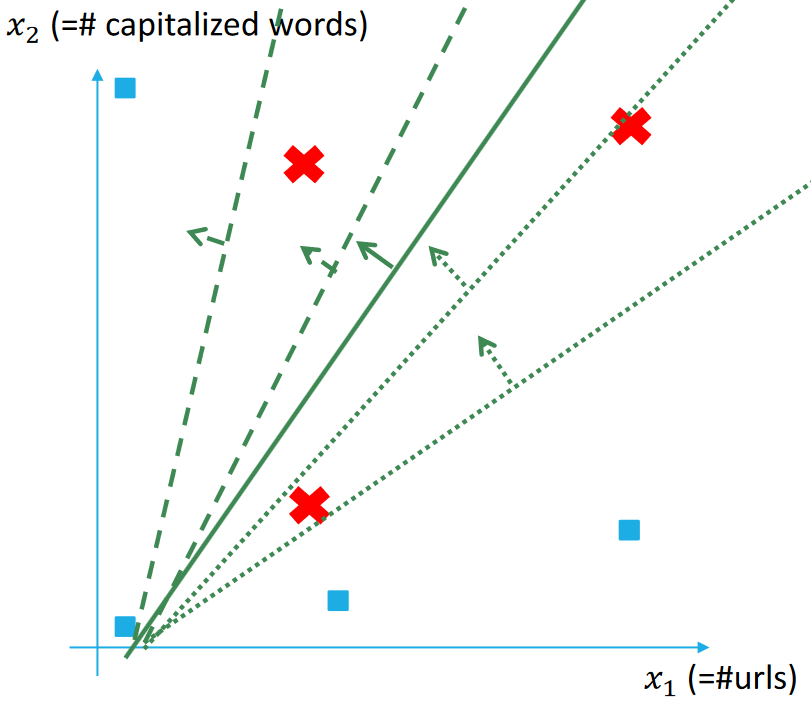
\includegraphics[width=0.3\linewidth]{./img/01_loss_spam.png}
            \caption{\parbox[t]{0.7\linewidth}{
                    Example of linear classifier for spam detection. 
                    Small changes on the boundary line do not change the 0-1 loss. 
                    The loss itself does not tell which is the best direction to move the line.
            }}
        \end{figure}


    \item[Root mean square error] \marginnote{Root mean square error}
        Loss computed as the direct comparison between the prediction and target label:
        \[ \mathcal{L}\big( \matr{\theta}, (\vec{x}^{(i)}, y^{(i)}) \big) = \Vert f(\vec{x}^{(i)}; \matr{\theta}) - y^{(i)} \Vert_2 \]
        Note that $y^{(i)}$ might be encoded (e.g. one-hot).


    \item[Cross-entropy loss] \marginnote{Cross-entropy loss}
        Transform the logits of a model into a probability distribution and estimate the parameters through MLE.

        \begin{descriptionlist}
            \item[Softmax] \marginnote{Softmax}
                Function that converts its input into a probability distribution.
                Given the logits $\vec{s} \in \mathbb{R}^{c}$, the score $\vec{s}_j$ of class $j$ is converted into a probability as follows:
                \[ 
                    \mathcal{P}_\text{model}(Y = j | X = \vec{x}^{(i)}; \matr{\theta}) = 
                        \texttt{softmax}_j(\vec{s}) = 
                        \frac{\exp(\vec{s}_j)}{\sum_{k=1}^{c} \exp(\vec{s}_k)} 
                \]

                For numerical stability, \texttt{softmax} is usually computed as:
                \[
                    \begin{split}
                        \texttt{softmax}_j(\vec{s} - \max\{ \vec{s} \}) &= \frac{\exp(\vec{s}_j - \max\{ \vec{s} \})}{\sum_{k=1}^{c} \exp(\vec{s}_k - \max\{ \vec{s} \})} \\
                        &= \frac{\cancel{\exp(- \max\{ \vec{s} \})}\exp(\vec{s}_j)}{\cancel{\exp(- \max\{ \vec{s} \})}\sum_{k=1}^{c} \exp(\vec{s}_k)} = \texttt{softmax}_j(\vec{s})
                    \end{split}    
                \]
            
            \item[Maximum likelihood estimation] \marginnote{Cross-entropy loss}
                Use MLE to estimate the parameters on the probability distribution outputted by the \texttt{softmax} function:
                \[
                    \begin{split}
                        \matr{\theta}^* &= \arg\max_\matr{\theta} \mathcal{P}_\text{model}(y^{(1)}, \dots, y^{(N)} | \vec{x}^{(1)}, \dots, \vec{x}^{(N)}; \matr{\theta}) \\
                            &= \arg\max_\matr{\theta} \prod_{i=1}^{N} \mathcal{P}_\text{model}(Y = y^{(i)} | X=\vec{x}^{(i)}; \matr{\theta}) \\
                            &= \arg\max_\matr{\theta} \sum_{i=1}^{N} \log\mathcal{P}_\text{model}(Y = y^{(i)} | X=\vec{x}^{(i)}; \matr{\theta}) \\
                            &= \arg\min_\matr{\theta} \sum_{i=1}^{N} -\log\mathcal{P}_\text{model}(Y = y^{(i)} | X=\vec{x}^{(i)}; \matr{\theta}) \\
                            &= \arg\min_\matr{\theta} \sum_{i=1}^{N} -\log\left( \frac{\exp(\vec{s}_{y^{(i)}})}{\sum_{k=1}^{c} \exp(\vec{s}_k)} \right) \\
                            &= \arg\min_\matr{\theta} \sum_{i=1}^{N} -\log\left( \exp(\vec{s}_{y^{(i)}}) \right) + \log\left( \sum_{k=1}^{c} \exp(\vec{s}_k) \right) \\
                            &= \arg\min_\matr{\theta} \sum_{i=1}^{N} -\vec{s}_{y^{(i)}} + \log\left( \sum_{k=1}^{c} \exp(\vec{s}_k) \right) \\
                    \end{split}    
                \]

                The second term ($\log\left( \sum_{k=1}^{c} \exp(\vec{s}_k)\right)$) is called \texttt{logsumexp} and approximates the max function.
                Therefore, the loss can be seen as:
                \[ 
                    \mathcal{L}\big( \matr{\theta}, (\vec{x}^{(i)}, y^{(i)}) \big) 
                    = -\vec{s}_{y^{(i)}} + \log\left( \sum_{k=1}^{c} \exp(\vec{s}_k) \right) 
                    \approx -\vec{s}_{y^{(i)}} + \max\{ \vec{s} \}
                \]
        \end{descriptionlist}
        
\end{description}


\subsection{Gradient descent}

\begin{description}
    \item[Gradient descent] \marginnote{Gradient descent}
        An epoch $e$ of gradient descent does the following:
        \begin{enumerate}
            \item Classify all training data to obtain the predictions $\hat{y}^{(i)} = f(\vec{x}^{(i)}; \matr{\theta}^{(e-1)})$
                and the loss $\mathcal{L}(\matr{\theta}^{(e-1)}, \matr{D}^\text{train})$.
            \item Compute the gradient $\nabla \mathcal{L} = \frac{\partial\mathcal{L}}{\partial \matr{\theta}} (\matr{\theta}^{(e-1)}, \matr{D}^\text{train})$.
            \item Update the parameters $\matr{\theta}^{(e)} = \matr{\theta}^{(e-1)} - \texttt{lr} \cdot \nabla \mathcal{L}$.
        \end{enumerate}

    \item[Stochastic gradient descent] \marginnote{Stochastic gradient descent}
        Reduce the computational cost of gradient descent by computing the gradient of a single sample.
        An epoch $e$ of SGD does the following:
        \begin{enumerate}
            \item Shuffle the training data $\matr{D}^\text{train}$.
            \item For $i = 0, \dots, N-1$:
            \begin{enumerate}
                \item Classify $\vec{x}^{(i)}$ to obtain the prediction $\hat{y}^{(i)} = f(\vec{x}^{(i)}; \matr{\theta}^{(e*N+i)})$
                and the loss $\mathcal{L}\big( \matr{\theta}^{(e*N+i)}, (\vec{x}^{(i)}, y^{(i)}) \big)$.
                \item Compute the gradient $\nabla \mathcal{L} = \frac{\partial\mathcal{L}}{\partial \matr{\theta}}\big( \matr{\theta}^{(e*N+i)}, (\vec{x}^{(i)}, y^{(i)}) \big)$.
                \item Update the parameters $\matr{\theta}^{(e*N+i+1)} = \matr{\theta}^{(e*N+i)} - \texttt{lr} \cdot \nabla \mathcal{L}$.
            \end{enumerate}
        \end{enumerate}

    \item[SGD with mini-batches] \marginnote{SGD with mini-batches}
        Increase the update accuracy of SGD by using a mini-batch.
        An epoch $e$ of SGD with mini-batches of size $B$ does the following:
        \begin{enumerate}
            \item Shuffle the training data $\matr{D}^\text{train}$.
            \item For $u = 0, \dots, U$, with $U = \lceil \frac{N}{B} \rceil$:
            \begin{enumerate}
                \item Classify the examples $\matr{X}^{(u)} = \{ \vec{x}^{(Bu)}, \dots, \vec{x}^{(B(u+1)-1)} \}$ 
                    to obtain the predictions $\hat{Y}^{(u)} = f(\vec{X}^{(u)}; \matr{\theta}^{(e*U+u)})$
                    and the loss $\mathcal{L}\big( \matr{\theta}^{(e*U+u)}, (\matr{X}^{(u)}, \hat{Y}^{(u)}) \big)$.
                \item Compute the gradient $\nabla \mathcal{L} = \frac{\partial\mathcal{L}}{\partial \matr{\theta}}\big( \matr{\theta}^{(e*U+u)}, (\matr{X}^{(u)}, \hat{Y}^{(u)}) \big)$.
                \item Update the parameters $\matr{\theta}^{(e*U+u+1)} = \matr{\theta}^{(e*U+u)} - \texttt{lr} \cdot \nabla \mathcal{L}$.
            \end{enumerate}
        \end{enumerate}

        The following properties generally hold:
        \begin{itemize}
            \item Larger batches provide a smoother estimation of the gradient and allow to better exploit parallel hardware (below a certain limit, there is no gain in time).
            \item Smaller batches require more iterations to train but might have a regularization effect for better generalization.
        \end{itemize}
\end{description}



\section{Linear classifier}
\marginnote{Linear classifier}

Determine the class by computing a linear combination of the input.

Given $c$ classes and a flattened image $\vec{x} \in \mathbb{R}^{i}$, a linear classifier $f$ parametrized on $\matr{W} \in \mathbb{R}^{c \times i}$ is defined as:
\[ f(\vec{x}; \matr{W}) = \matr{W}\vec{x} = \texttt{logits} \]
where the $\texttt{logits} \in \mathbb{R}^{c}$ vector contains a score for each class.

The prediction is obtained as the index of the maximum score.

\begin{remark}
    Predicting directly the integer encoded classes is not ideal as it would give a (probably) inexistent semantic ordering
    (e.g. if $2$ encodes bird and $3$ encodes cat, $2.5$ should not mean half bird and half cat).
\end{remark}

\begin{remark}
    Linear classifiers can be seen as a template-matching method.
    Each row of $\matr{W} \in \mathbb{R}^{c \times i}$ is a class template that is cross-correlated with the image to obtain a score.
\end{remark}

\marginnote{Affine classifier}
In practice, a linear classifier is actually an affine classifier parametrized on $\theta = (\matr{W} \in \mathbb{R}^{c \times i}, \vec{b} \in \mathbb{R}^{c})$:
\[ f(\vec{x}; \theta) = \matr{W}\vec{x} + \vec{b} = \texttt{logits} \]